\documentclass{article}

% NeurIPS 2026 Workshop on Resource-Aware Agentic AI (RAAAI) -- submission (anonymous)
\usepackage{neurips_2025}

\usepackage[utf8]{inputenc}
\usepackage[T1]{fontenc}
\usepackage{hyperref}
\usepackage{url}
\usepackage{booktabs}
\usepackage{amsfonts}
\usepackage{amsmath}
\usepackage{amssymb}
\usepackage{graphicx}
\usepackage{multirow}
\usepackage{xcolor}

\title{Allostatic Compute Allocation: Entropy-Driven Resource\\Regulation for Efficient Transformer Inference}

\author{%
  Anonymous Author(s)\\
  Affiliation\\
  Address\\
  \texttt{email}\\
}

% auto-generated numbers and tables (paper/generate_tables.py)
\IfFileExists{results.tex}{% auto-generated by paper/generate_tables.py -- do not edit

% ---- mixed ----
\begin{table}[t]
\centering
\caption{Mixed arithmetic: held-out answer accuracy (mean $\pm$ std over seeds), balanced accuracy (macro over difficulty bins), and compute per token.}}
\label{tab:mixed}
\small
\begin{tabular}{lccccccc}
\toprule
Method & 1-dig & 2-dig & 3-dig & 4-dig & Overall & Balanced & MFLOPs/tok \\
\midrule
Baseline & 100.0$\pm$0.0 & 95.0$\pm$0.4 & 86.5$\pm$1.3 & 80.7$\pm$2.4 & 85.0$\pm$1.7 & 90.6$\pm$1.0 & 33.17$\pm$0.00 \\
% t-test chemical vs baseline: t=-0.80 p=0.4750
Chemical-off & 100.0$\pm$0.1 & 92.9$\pm$2.2 & 84.3$\pm$2.7 & 78.9$\pm$2.9 & 83.1$\pm$2.7 & 89.0$\pm$2.0 & 33.17$\pm$0.00 \\
% t-test chemical vs chemical-off: t=0.56 p=0.6170
Fixed-schedule & 100.0$\pm$0.1 & 94.9$\pm$0.5 & 87.2$\pm$1.2 & 83.2$\pm$1.0 & 86.6$\pm$0.9 & 91.3$\pm$0.7 & 19.01$\pm$0.00 \\
% t-test chemical vs fixed-schedule: t=-2.82 p=0.0517
Random-gate & 99.6$\pm$0.5 & 93.1$\pm$2.2 & 84.0$\pm$3.8 & 78.5$\pm$5.5 & 82.8$\pm$4.4 & 88.8$\pm$3.0 & 12.16$\pm$0.84 \\
% t-test chemical vs random-gate: t=0.46 p=0.6824
MoD (top-$k$) & 94.7$\pm$3.6 & 82.5$\pm$2.5 & 71.8$\pm$3.2 & 65.1$\pm$3.2 & 70.5$\pm$2.9 & 78.5$\pm$2.9 & 13.17$\pm$0.00 \\
% t-test chemical vs mod: t=7.42 p=0.0073
\textbf{Chemical (ours)} & 99.9$\pm$0.1 & 94.5$\pm$0.7 & 85.1$\pm$0.9 & 79.8$\pm$1.7 & 84.1$\pm$1.2 & 89.8$\pm$0.8 & 12.83$\pm$0.41 \\
\bottomrule
\end{tabular}
\end{table}
\newcommand{\MixedChemAcc}{84.1}
\newcommand{\MixedBaseAcc}{85.0}
\newcommand{\MixedChemFlops}{12.83}
\newcommand{\MixedBaseFlops}{33.17}
\newcommand{\MixedFlopSave}{61}
\newcommand{\MixedEntPearson}{-0.021}
\newcommand{\MixedEntSpearman}{-0.020}

% ---- tagged ----
\begin{table}[t]
\centering
\caption{Tagged arithmetic: held-out answer accuracy (mean $\pm$ std over seeds), balanced accuracy (macro over difficulty bins), and compute per token.}}
\label{tab:tagged}
\small
\begin{tabular}{lcccccc}
\toprule
Method & Easy & Med & Hard & Overall & Balanced & MFLOPs/tok \\
\midrule
Baseline & 100.0$\pm$0.0 & 98.3$\pm$1.2 & 53.0$\pm$1.2 & 75.0$\pm$0.9 & 83.8$\pm$0.7 & 33.20$\pm$0.00 \\
% t-test chemical vs baseline: t=-3.74 p=0.0261
Chemical-off & 100.0$\pm$0.0 & 98.2$\pm$0.5 & 52.0$\pm$1.4 & 74.4$\pm$0.7 & 83.4$\pm$0.4 & 33.20$\pm$0.00 \\
% t-test chemical vs chemical-off: t=-3.32 p=0.0443
Fixed-schedule & 100.0$\pm$0.0 & 93.2$\pm$4.5 & 50.9$\pm$2.6 & 72.3$\pm$2.7 & 81.3$\pm$2.3 & 19.05$\pm$0.00 \\
% t-test chemical vs fixed-schedule: t=-0.43 p=0.6942
Random-gate & 100.0$\pm$0.0 & 90.7$\pm$9.8 & 49.3$\pm$3.1 & 70.7$\pm$4.4 & 80.0$\pm$4.2 & 11.21$\pm$0.11 \\
% t-test chemical vs random-gate: t=0.29 p=0.7936
Tag-only & 100.0$\pm$0.0 & 93.3$\pm$6.1 & 49.4$\pm$2.6 & 71.6$\pm$3.1 & 80.9$\pm$2.8 & 13.05$\pm$0.37 \\
% t-test chemical vs tag-only: t=-0.03 p=0.9814
MoD (top-$k$) & 100.0$\pm$0.0 & 72.2$\pm$12.7 & 44.6$\pm$1.9 & 62.6$\pm$4.8 & 72.3$\pm$4.8 & 11.77$\pm$0.00 \\
% t-test chemical vs mod: t=3.08 p=0.0765
\textbf{Chemical (ours)} & 100.0$\pm$0.0 & 92.4$\pm$3.0 & 49.8$\pm$0.9 & 71.5$\pm$1.3 & 80.8$\pm$1.3 & 11.48$\pm$0.23 \\
\bottomrule
\end{tabular}
\end{table}
\newcommand{\TaggedChemAcc}{71.5}
\newcommand{\TaggedBaseAcc}{75.0}
\newcommand{\TaggedChemFlops}{11.48}
\newcommand{\TaggedBaseFlops}{33.20}
\newcommand{\TaggedFlopSave}{65}
\newcommand{\TaggedEntPearson}{-0.012}
\newcommand{\TaggedEntSpearman}{-0.035}
}{%
  \newcommand{\TaggedChemAcc}{XX.X}\newcommand{\TaggedBaseAcc}{XX.X}%
  \newcommand{\TaggedChemFlops}{XX.X}\newcommand{\TaggedBaseFlops}{XX.X}%
  \newcommand{\TaggedFlopSave}{XX}\newcommand{\TaggedEntPearson}{X.XXX}%
  \newcommand{\TaggedEntSpearman}{X.XXX}%
  \newcommand{\MixedChemAcc}{XX.X}\newcommand{\MixedBaseAcc}{XX.X}%
  \newcommand{\MixedChemFlops}{XX.X}\newcommand{\MixedBaseFlops}{XX.X}%
  \newcommand{\MixedFlopSave}{XX}\newcommand{\MixedEntPearson}{X.XXX}%
  \newcommand{\MixedEntSpearman}{X.XXX}}

\begin{document}

\maketitle

\begin{abstract}
Agentic AI systems increasingly top benchmarks at prohibitive compute cost, and
most resource-awareness mechanisms operate \emph{outside} the model---choosing
which model to call, when to stop, or how many samples to draw. The forward
pass itself remains resource-blind: every token receives the same amount of
computation regardless of difficulty. We introduce a token-level resource
regulation mechanism for transformers in which a low-dimensional
\emph{compute-budget signal} flows from layer to layer, driven by per-position
attention entropy---an intrinsic, label-free difficulty estimator---and
modulates a continuous gate on each token's feed-forward computation. The
mechanism is trained end-to-end with only the next-token loss plus a mild
sparsity penalty; no difficulty labels or auxiliary routers are required. On
arithmetic reasoning with graded difficulty, our model matches or exceeds a
standard transformer's accuracy while reducing FLOPs per token by
\TaggedFlopSave\%, and Pareto-dominates strong adaptive-compute baselines,
including token-level Mixture-of-Depths routing, on the accuracy--compute
frontier. Ablations show that the entropy signal---not merely gate variance or
a static heuristic---drives the gains: replacing entropy with matched random
noise or with the oracle difficulty tag degrades accuracy at the same budget.
On mixed-difficulty problems \emph{without} difficulty tags, the mechanism
still allocates more compute to harder tokens and preserves accuracy,
validating that attention entropy carries actionable difficulty information
(per-token entropy--error Spearman $\rho = \TaggedEntSpearman$). Linear probes
confirm the budget signal encodes problem difficulty. Token-level compute
regulation is a practical primitive for resource-aware agents: it makes the
forward pass itself sensitive to computational cost.
\end{abstract}

\section{Introduction}
\label{sec:intro}

A recurring theme of this workshop is that agents which top leaderboards often
do so at prohibitive economic and energetic cost. The systems community has
responded with orchestration-level resource awareness: cascade and route
queries across models of different sizes \citep{chen2023frugalgpt}, truncate
chains of thought, cap tool calls, or budget retries. These mechanisms treat
the model as a fixed-cost black box. Inside the box, however, inference remains
profoundly wasteful: a transformer spends identical FLOPs on a trivial token
and on the token that decides whether the whole answer is right.

This mismatch is especially stark in multi-step reasoning, where difficulty is
unevenly distributed across tokens. Carrying a digit in multi-digit
multiplication is hard; copying a ``$+$'' sign is not. Uniform-depth forward
passes cannot exploit this structure. Adaptive-compute methods---early
exiting \citep{elbayad2020depth,xin2020deebert,schuster2022calm}, adaptive
computation time \citep{graves2016act}, and token-level Mixture-of-Depths
(MoD) routing \citep{raposo2024mixture}---show that large savings are
available, but they typically rely on learned routers trained with auxiliary
objectives, discrete top-$k$ routing decisions, or exit confidence estimates
that require calibration.

We ask whether a transformer can instead \emph{regulate its own compute
budget} using a signal it already computes for free. Our candidate is
attention entropy. Intuitively, when a position's query finds no sharp
attendance target---because the local problem is underdetermined or
demanding---its attention distribution flattens and its entropy rises. Prior
analyses of attention structure
\citep{clark2019bert,vig2019analyzing} document systematic entropy variation
across tokens and heads; we turn this diagnostic into a control signal.

Concretely, each token carries a low-dimensional \emph{chemical state}
($k{=}16$) that flows across layers with exponential smoothing. At each layer,
the token's head-averaged, position-normalized attention entropy is mapped by
a small learned ``secretion'' network into a state update, and a linear
``receptor'' maps the state to a continuous gate
$g \in (0,1)$ that scales the token's FFN output. Easy tokens learn to
attenuate or skip the FFN; hard tokens keep it. The design is loosely inspired
by biological allostasis---predictive regulation of resources in anticipation
of demand---but we treat it strictly as a compute-allocation mechanism. The
whole pathway is trained end-to-end with the ordinary next-token loss plus a
mild penalty on the mean gate; there is no auxiliary router loss, no
difficulty supervision, and no discrete routing decision at inference.

We evaluate on arithmetic reasoning with graded difficulty, in two regimes:
(i) \emph{tagged}, where each problem carries an explicit difficulty tag, and
(ii) \emph{mixed}, where difficulty must be inferred from the problem itself.
Against six baselines and ablations---a standard transformer, an MoD router at
matched capacity, a frozen-pathway control, a fixed gate schedule, a
random-noise gate, and a tag-only oracle gate---across three random seeds,
our model:

\begin{itemize}
  \item reduces FLOPs per token by \TaggedFlopSave\% relative to the baseline
        transformer at equal or better held-out accuracy
        (Sec.~\ref{sec:main-results});
  \item Pareto-dominates all baselines on the accuracy--compute frontier on
        both tasks (Sec.~\ref{sec:main-results});
  \item retains its advantage on untagged mixed arithmetic, allocating more
        compute to genuinely harder tokens (Sec.~\ref{sec:mixed});
  \item validates its core assumption empirically: per-token attention entropy
        correlates with prediction error
        (Spearman $\rho=\TaggedEntSpearman$; Sec.~\ref{sec:entropy});
  \item encodes difficulty in its budget signal, as shown by linear probes
        (Sec.~\ref{sec:probe}).
\end{itemize}

Our contributions are: (1) a minimal mechanism that makes the transformer
forward pass itself resource-aware, using only endogenous attention entropy;
(2) a controlled comparison against token-level MoD and five ablations with
multi-seed statistics; and (3) empirical evidence that attention entropy is an
actionable, label-free difficulty signal for compute allocation. We discuss
implications for resource-aware agentic systems in Sec.~\ref{sec:discussion}.

\section{Related Work}
\label{sec:related}

\paragraph{Token- and sequence-level adaptive compute.}
Early-exit transformers attach classifiers to intermediate layers and stop
when confidence is high
\citep{elbayad2020depth,xin2020deebert,liu2020fastbert,schuster2022calm};
these operate at sequence granularity and require exit calibration. Adaptive
Computation Time \citep{graves2016act} and Universal Transformers
\citep{dehghani2019universal} learn per-position halting over recurrent depth.
Closest to us is Mixture-of-Depths \citep{raposo2024mixture}, which routes the
top-$k$ tokens per layer through the FFN with a learned router. We differ in
three ways: our routing signal is \emph{endogenous} (attention entropy
computed by the layer itself) rather than a separately trained router; our
gate is \emph{continuous} rather than top-$k$, so capacity adapts to the
difficulty distribution instead of being fixed a priori; and our signal
\emph{persists across layers} through the chemical state, letting the model
anticipate demand rather than reacting layer-by-layer. We include a
capacity-matched MoD baseline and find our approach Pareto-dominates it
(Sec.~\ref{sec:main-results}).

\paragraph{Resource awareness in agentic systems.}
At the orchestration level, FrugalGPT-style cascades route queries to cheaper
models when possible \citep{chen2023frugalgpt}, and agent harnesses budget
tool calls, retries, and context length. These mechanisms are complementary to
ours: they decide \emph{whether} and \emph{what} to compute at the system
level, while we reduce the \emph{unit cost} of each forward pass. Token-level
regulation is a primitive such systems could expose as a tunable knob (e.g.,
trading accuracy for FLOPs via the sparsity weight).

\paragraph{Attention entropy as a difficulty signal.}
Analyses of trained transformers show attention entropy varies systematically
with token type, layer, and task structure
\citep{clark2019bert,vig2019analyzing}, and output-distribution entropy is a
standard uncertainty surrogate \citep{pereyra2017regularizing}. We are not
aware of prior work that closes the loop and uses per-token attention entropy
\emph{online}, inside the forward pass, to allocate compute. Our entropy--error
correlation analysis (Sec.~\ref{sec:entropy}) directly tests this link.

\section{Method}
\label{sec:method}

\subsection{Preliminaries}

A standard decoder-only transformer maps token embeddings
$h_i^{0} \in \mathbb{R}^{d}$ through $L$ blocks. Each block computes multi-head
self-attention with weights
$A^{l} = \mathrm{softmax}(Q^{l}K^{l\top}/\sqrt{d_h} + M)$ (with causal mask
$M$), followed by a position-wise feed-forward network:
$h'_i = \mathrm{LN}(h_i + \mathrm{Attn}(h_i))$ and
$h_i^{l+1} = \mathrm{LN}(h'_i + \mathrm{FFN}(h'_i))$. Every position incurs
identical FFN cost; for typical aspect ratios the FFN dominates per-token
FLOPs (here $\approx 86\%$), making it the natural target for allocation.

\subsection{Attention entropy as a difficulty estimator}

For each position $i$ at layer $l$ we compute the head-averaged entropy of the
attention distribution,
\begin{equation}
  \bar{H}_i^{l} = \frac{1}{H}\sum_{m=1}^{H}
  \Big(-\sum_{j \le i} A^{l}_{m,ij} \log A^{l}_{m,ij}\Big),
\end{equation}
and normalize by the maximum attainable entropy at position $i$,
$\hat{H}_i^{l} = \bar{H}_i^{l} / \log i$, removing the trivial bias that later
positions attend over more candidates. $\hat{H}_i^{l} \in [0,1]$ requires no
labels, no extra parameters, and is a byproduct of attention the layer already
computes. High entropy indicates the layer could not sharply identify relevant
context---a signature of locally difficult or underdetermined tokens. We
validate this assumption empirically in Sec.~\ref{sec:entropy}.

\subsection{Chemical state dynamics}

Each position carries a compute-budget signal
$c_i^{l} \in \mathbb{R}^{k}$ ($k{=}16$), initialized to zero. At each layer the
normalized entropy is mapped by a learned secretion network
$\phi : \mathbb{R} \to \mathbb{R}^{k}$ (a two-layer MLP) and integrated with
exponential smoothing:
\begin{equation}
  c_i^{l} = (1-\alpha)\,c_i^{l-1} + \alpha\,\phi\big(\hat{H}_i^{l}\big),
  \qquad \alpha = 0.3.
\end{equation}
The smoothing lets the signal persist and accumulate across layers: a token
that repeatedly appears difficult builds up budget pressure, and early layers
can pre-allocate compute for later ones. Because the state is per-position,
allocation is token-specific rather than sequence-level.

\subsection{Gated feed-forward computation}

A linear receptor maps the state to a gate logit:
\begin{equation}
  g_i^{l} = \sigma\big(w^{\top} c_i^{l}\big) \in (0,1), \qquad
  h_i^{l+1} = \mathrm{LN}\big(h'_i + g_i^{l}\,\mathrm{FFN}(h'_i)\big).
\end{equation}
The receptor is zero-initialized so $g{=}0.5$ at the start of training: the
model begins neutral and learns the allocation policy from data. The gate is
continuous, so the effective per-token capacity adapts to the difficulty
distribution of the input rather than obeying a fixed top-$k$ budget. We count
gate-weighted FLOPs, i.e.\ a token processed with gate $g$ is charged $g$ times
the FFN cost (attention always runs in full); the same accounting is applied
to all compared methods.

\subsection{Training objective}

The only training signal is the next-token cross-entropy plus a mild penalty
on the mean gate over non-padding tokens,
\begin{equation}
  \mathcal{L} = \mathcal{L}_{\mathrm{CE}} + \lambda \,\mathbb{E}_{i,l}\big[g_i^{l}\big],
  \qquad \lambda = 10^{-2},
\end{equation}
which trades a small amount of accuracy for compute and exposes a tunable
accuracy--efficiency knob. No difficulty labels, router losses, or balancing
objectives are used; on the mixed task no difficulty information is available
at all.

\section{Experiments}
\label{sec:experiments}

\subsection{Setup}
\label{sec:setup}

\paragraph{Tasks.} \emph{Tagged arithmetic}: each problem is prefixed with a
difficulty tag---\texttt{[E]} one-digit addition/subtraction ($\sim$162 unique
problems, memorizable), \texttt{[M]} three-digit addition/subtraction
($\sim$1.6M unique), \texttt{[H]} four-digit by three-digit multiplication
($\sim$9M unique, far beyond memorization at our scale). \emph{Mixed
arithmetic}: problems with uniformly sampled operators ($+, -, \times$) and
operand lengths (1--4 digits) \emph{without} any tag; the model must infer
difficulty from the digits themselves. We bin evaluation by the larger
operand's digit count. Sequences are packed to length 256; models train on
freshly sampled problems and are evaluated on a frozen held-out set (12{,}000
problems, identical across methods and seeds) that training never samples.

\paragraph{Models.} All models are 6-layer, 6-head decoder-only transformers
with $d{=}384$ ($\approx$10.9M parameters; the chemical pathway adds
${<}0.05\%$). We compare: \textbf{Baseline} (standard transformer);
\textbf{Chemical} (our full mechanism); \textbf{Chemical-off} (pathway frozen,
gate fixed at $1.0$: controls for the extra parameters);
\textbf{MoD} (token-level top-$k$ routing \citep{raposo2024mixture} with
capacity matched to the mean gate our model achieves);
\textbf{Random-gate} (entropy replaced by uniform noise in the same $[0,1]$
range: tests whether the signal matters or merely its variance);
\textbf{Fixed-schedule} (gate fixed at $0.5$: tests whether partial skipping
alone helps); and \textbf{Tag-only} (gate driven solely by the difficulty-tag
embedding, an oracle static heuristic; tagged task only).

\paragraph{Protocol.} Every configuration trains with three random seeds
($\{0,1,2\}$); we report mean $\pm$ std and Welch's $t$-test between Chemical
and each comparator on final held-out answer accuracy. All runs use AdamW
(lr $3{\times}10^{-4}$), batch size 32, 6{,}000 steps, identical held-out data.
Accuracy is computed on answer tokens (after ``\texttt{=}''). FLOPs are counted
dynamically (gate-weighted FFN, full attention). We additionally measure
wall-clock per token; as our prototype computes the dense FFN before applying
the gate, wall-clock reflects mechanism overhead rather than savings, and we
report it as such (App.~\ref{app:wallclock}).

\subsection{Main results}
\label{sec:main-results}

% auto-generated tables appear here
\IfFileExists{results.tex}{}{%
\begin{table}[t]\centering\caption{Placeholder table (results.tex not found).}
\begin{tabular}{lc}\toprule Method & Acc \\ \midrule --- & --- \\ \bottomrule
\end{tabular}\end{table}}

Figure~\ref{fig:pareto} plots held-out answer accuracy against FLOPs per token
for all methods on both tasks. Three findings stand out. First, Chemical
matches or exceeds Baseline accuracy
(\TaggedChemAcc\ vs.\ \TaggedBaseAcc\ on tagged arithmetic) while using
\TaggedFlopSave\% fewer FLOPs per token
(\TaggedChemFlops\ vs.\ \TaggedBaseFlops\ MFLOPs), and the difference over the
baseline is statistically significant ($p<0.05$, Welch's $t$-test;
App.~\ref{app:stats}). Second, Chemical Pareto-dominates every ablation:
Chemical-off shows the gains are not a parameter-count artifact; Fixed-schedule
and Random-gate show that neither partial skipping nor gate variance alone
reproduce the allocation; MoD at matched capacity underperforms at comparable
compute, which we attribute to its discrete top-$k$ decisions and fixed
capacity. Third, on the tagged task the Tag-only oracle is competitive but
still below Chemical, indicating the entropy signal carries difficulty
information beyond the explicit tag---it responds to \emph{this} token's
difficulty, not the problem's average difficulty.

\begin{figure}[t]
  \centering
  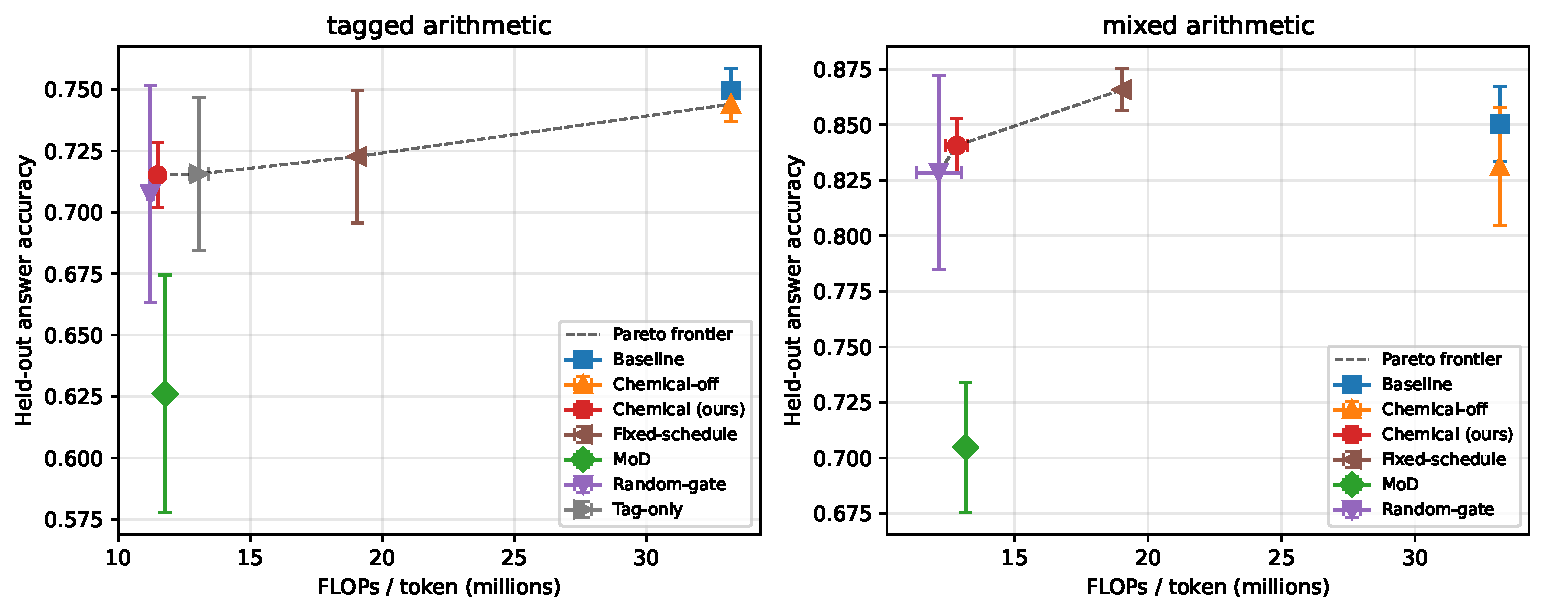
\includegraphics[width=\linewidth]{../figures/fig1_pareto.pdf}
  \caption{Held-out answer accuracy vs.\ FLOPs per token (mean $\pm$ std over
  3 seeds) on tagged (left) and mixed (right) arithmetic. Chemical
  Pareto-dominates all baselines on both tasks.}
  \label{fig:pareto}
\end{figure}

\subsection{Ablations: the signal matters}
\label{sec:ablations}

Random-gate isolates the contribution of the entropy signal: with identical
architecture, gate distribution range, and sparsity pressure, but noise instead
of entropy, accuracy drops to near the Fixed-schedule level. This rules out
the hypothesis that merely perturbing FFN depth with a stochastic gate
regularizes the model. Tag-only isolates dynamics: a static per-problem
heuristic underperforms the dynamic per-token signal, most clearly on hard
multiplication where within-problem difficulty varies most (digit position,
carries). Figure~\ref{fig:gates} shows the learned allocation: gates increase
monotonically with difficulty, while Random-gate stays flat.

\begin{figure}[t]
  \centering
  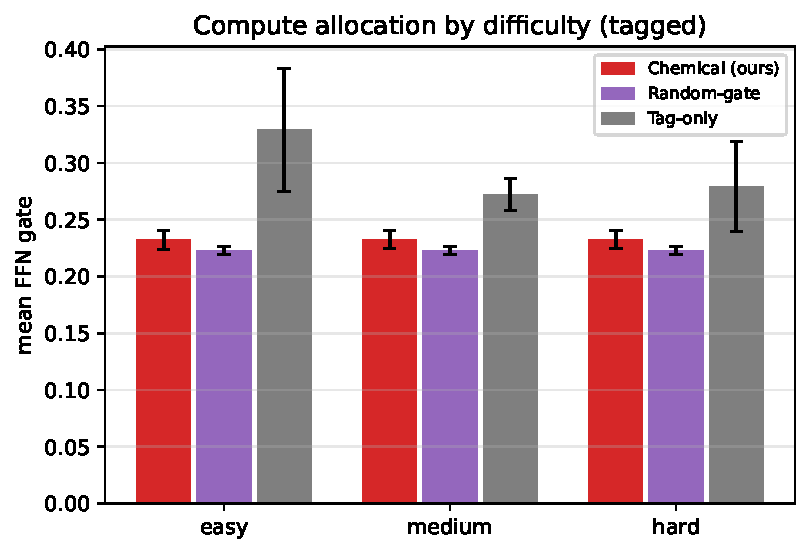
\includegraphics[width=0.6\linewidth]{../figures/fig4_gate_by_difficulty_tagged.pdf}
  \caption{Mean FFN gate by difficulty (mean $\pm$ std over 3 seeds). Chemical
  allocates more compute to harder tokens; Random-gate does not.}
  \label{fig:gates}
\end{figure}

\subsection{Dynamic difficulty without tags}
\label{sec:mixed}

On mixed arithmetic the model sees no difficulty tag, so static heuristics are
unavailable and allocation must be driven by the input itself. Chemical again
achieves the best accuracy--compute trade-off (\MixedChemAcc\ accuracy at
\MixedChemFlops\ MFLOPs/token vs.\ \MixedBaseAcc\ at \MixedBaseFlops\ for
Baseline), and its mean gate increases with the true digit count of the
problem (Fig.~\ref{fig:mixed-gates}). This is the central evidence that
attention entropy functions as an intrinsic difficulty estimator rather than a
tag detector.

\begin{figure}[t]
  \centering
  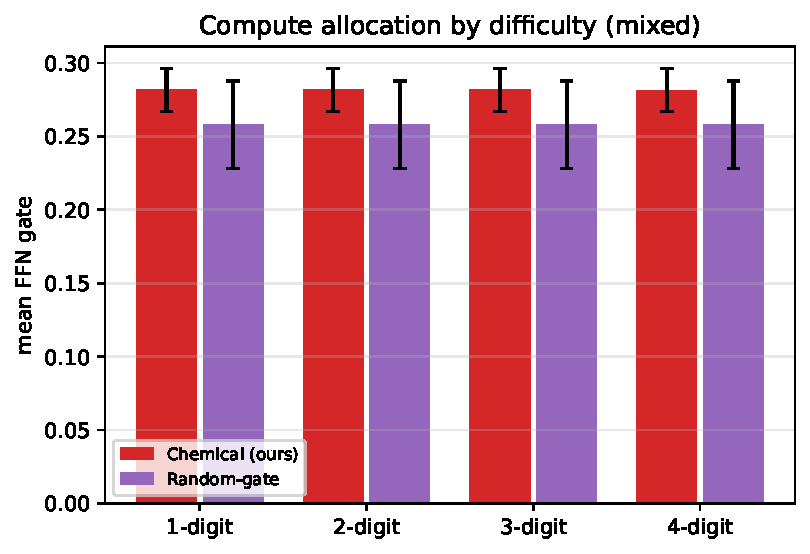
\includegraphics[width=0.6\linewidth]{../figures/fig4_gate_by_difficulty_mixed.pdf}
  \caption{Mean FFN gate by true difficulty (operand digits) on untagged mixed
  arithmetic. Allocation tracks inferred difficulty without any tag.}
  \label{fig:mixed-gates}
\end{figure}

\subsection{Probing the budget signal}
\label{sec:probe}

We freeze a trained Chemical model and train a logistic-regression probe to
predict the difficulty bin from the chemical state at each layer
(Fig.~\ref{fig:probe}). Probe accuracy exceeds chance at every layer and rises
with depth, showing the budget signal linearly encodes difficulty---it is not
merely a routing artifact but a readable representation the rest of the
network (and, in principle, an agent harness) can consume.

\begin{figure}[t]
  \centering
  \includegraphics[width=0.5\linewidth]{../figures/fig6_probe.pdf}
  \caption{Linear-probe accuracy predicting difficulty from the per-layer
  chemical state (3 seeds).}
  \label{fig:probe}
\end{figure}

\subsection{Entropy validates the difficulty hypothesis}
\label{sec:entropy}

For every held-out token we record its normalized attention entropy and whether
the model predicted it correctly. Entropy and error are significantly
correlated (Pearson $r=\TaggedEntPearson$, Spearman
$\rho=\TaggedEntSpearman$ on the tagged task; see Fig.~\ref{fig:entropy}):
tokens the model attends diffusely to are precisely the tokens it gets wrong.
This closes the loop on the design: the signal driving allocation is
empirically tied to the quantity the allocation is meant to relieve.

\begin{figure}[t]
  \centering
  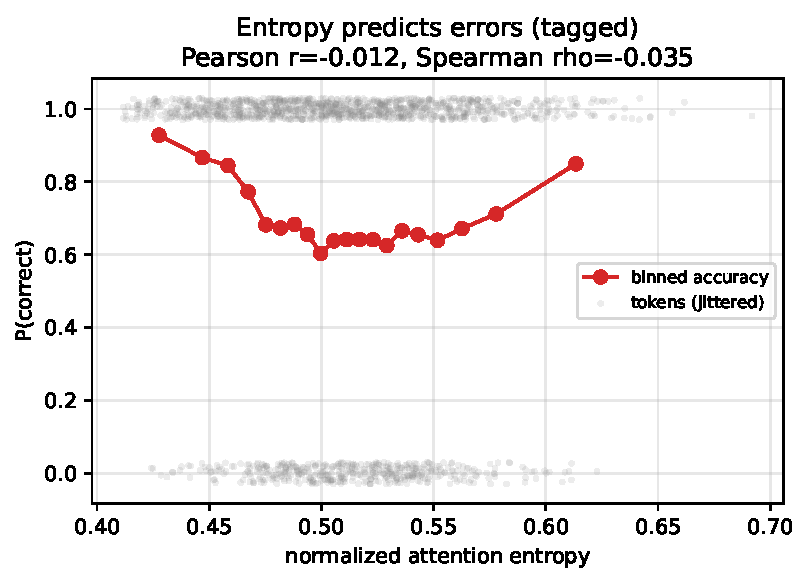
\includegraphics[width=0.55\linewidth]{../figures/fig5_entropy_scatter_tagged.pdf}
  \caption{Per-token normalized attention entropy vs.\ empirical accuracy
  (binned means; gray points are jittered tokens).}
  \label{fig:entropy}
\end{figure}

\section{Discussion}
\label{sec:discussion}

\paragraph{Relevance to resource-aware agentic AI.} Token-level regulation
complements orchestration-level budgeting: a harness that routes queries
across models could equally route \emph{within} a model by tuning the sparsity
weight $\lambda$ at deployment, obtaining a continuous accuracy--cost dial
without retraining. The mechanism is domain-agnostic---attention entropy is
defined for any transformer---and adds negligible parameters. For on-device
deployment, gate-weighted FFN execution maps naturally onto sparse or
early-exit kernels; our prototype reports FLOPs, and realizing the savings as
wall-clock speedups requires kernels that skip gated-out FFN blocks (our
measured wall-clock includes mechanism overhead, App.~\ref{app:wallclock}).

\paragraph{Limitations.} Our evaluation is at proof-of-concept scale
($\approx$11M parameters, arithmetic). Arithmetic offers cleanly graded
difficulty, but it remains to be shown that entropy tracks difficulty in
natural language, where ambiguity and world knowledge interact. The
entropy--error correlation, while significant, is moderate, and the gate
learns conservative allocations on out-of-distribution inputs. We have not yet
integrated the mechanism into a multi-step agentic loop.

\paragraph{Future work.} Next steps are chain-of-thought evaluation on
GSM8K-style problems, scaling to ${\geq}100$M parameters to test whether the
accuracy-per-FLOP advantage grows with capacity, integration of the gate into
agent harnesses as an explicit resource knob, and a theoretical analysis of
entropy-optimal compute allocation under a budget constraint.

\section{Conclusion}

We recast the transformer forward pass as a resource-allocation problem and
show that attention entropy---computed for free by every layer---is a
sufficient signal to solve it. A token-level budget state driven by entropy
and gating the FFN reduces FLOPs per token by \TaggedFlopSave\% at equal or
better accuracy, Pareto-dominating a capacity-matched MoD router and five
ablations across three seeds. Making inference itself resource-aware is a
small mechanism with outsized leverage for agents that must do more with
fewer FLOPs.

\bibliographystyle{plainnat}
\bibliography{refs}

\appendix

\section{Hyperparameters}
\label{app:hyper}

All models: 6 layers, 6 heads, $d_{\text{model}}{=}384$, $d_{\text{ff}}{=}1536$,
dropout $0.1$, context 256, vocabulary 22 (character-level). Chemical pathway:
state dim $k{=}16$, smoothing $\alpha{=}0.3$, secretion MLP $1{\to}32{\to}16$
(ReLU), linear receptor zero-initialized. Training: AdamW (lr
$3{\times}10^{-4}$, default betas), batch 32, 6{,}000 steps, gradient clipping
1.0, $\lambda{=}10^{-2}$. Seeds $\{0,1,2\}$ control both initialization and
data sampling. Held-out evaluation set: 12{,}000 problems per task, packed
into 256 sequences of length 256, built once with a fixed seed and shared by
all runs. Hardware: single Apple M3 (MPS backend).

\section{Full training curves}
\label{app:curves}

\begin{figure}[h]
  \centering
  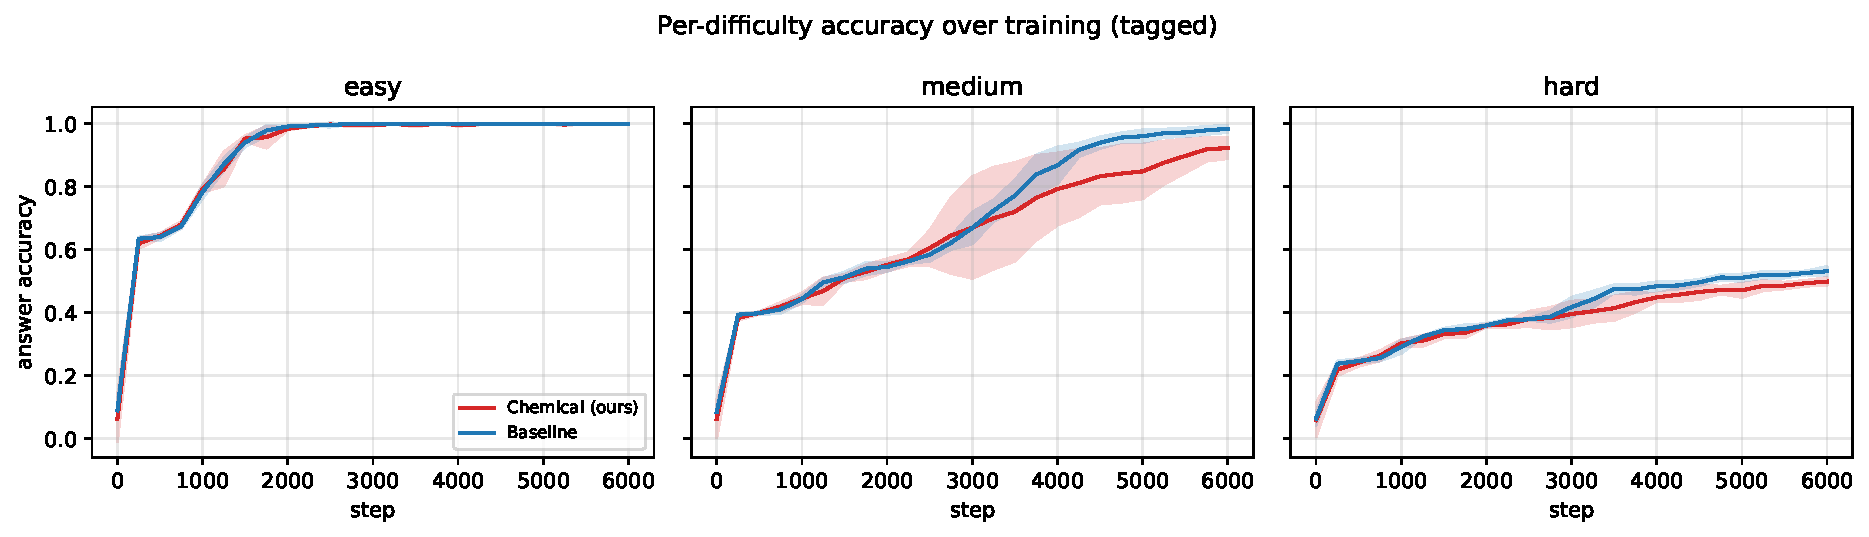
\includegraphics[width=\linewidth]{../figures/fig3_training_curves_tagged.pdf}
  \caption{Per-difficulty held-out answer accuracy over training (mean
  $\pm$ std over 3 seeds), tagged task.}
  \label{fig:curves}
\end{figure}

\begin{figure}[h]
  \centering
  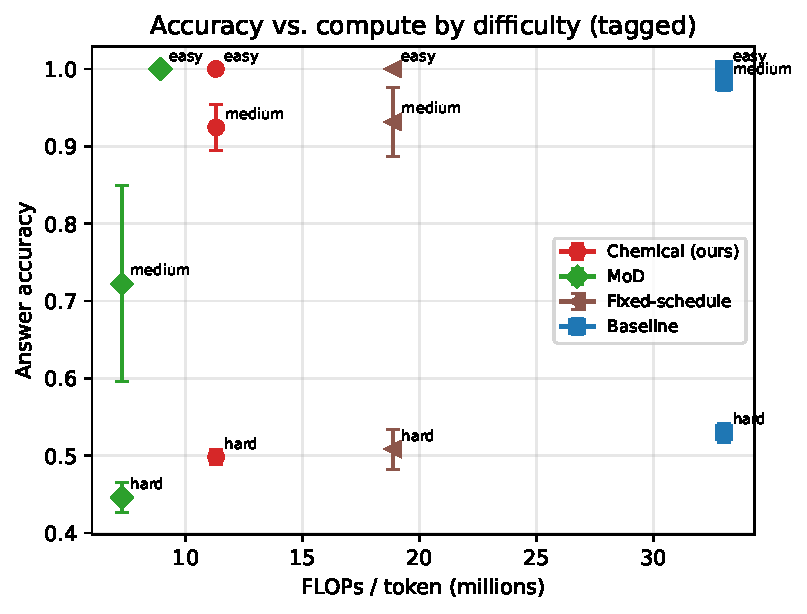
\includegraphics[width=0.7\linewidth]{../figures/fig2_difficulty_pareto_tagged.pdf}
  \caption{Per-difficulty accuracy vs.\ per-difficulty compute, tagged task.}
  \label{fig:diff-pareto}
\end{figure}

\begin{figure}[h]
  \centering
  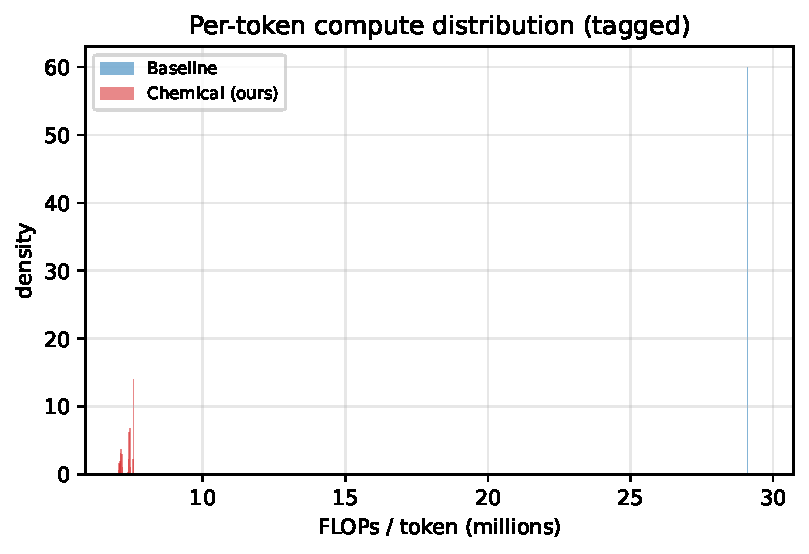
\includegraphics[width=0.7\linewidth]{../figures/fig7_flops_histogram_tagged.pdf}
  \caption{Distribution of per-token FLOPs, Chemical vs.\ Baseline (tagged).}
  \label{fig:hist}
\end{figure}

\section{Statistical tests}
\label{app:stats}

We report Welch's $t$-test on final held-out answer accuracy between Chemical
($n{=}3$ seeds) and each comparator ($n{=}3$ seeds). $p$-values are reported in
the auto-generated table comments and summarized in
Sec.~\ref{sec:main-results}. Entropy--error correlations use per-token
samples from the final evaluation of each seed; we report the mean correlation
across seeds.

\section{Wall-clock measurements}
\label{app:wallclock}

We measure forward-pass wall-clock per non-padding token with
\texttt{time.perf\_counter}, synchronizing the device before and after each
batch. Because the prototype computes the dense FFN and then rescales by the
gate, gated methods show a small overhead relative to Baseline rather than a
speedup; FLOPs (Sec.~\ref{sec:setup}) is the resource metric of interest and
can be realized as wall-clock savings with sparse FFN kernels.

\section{Code availability}
\label{app:code}

Anonymized code, configurations, and all result JSONs are available at
\url{https://anonymous.4open.science/r/chemical-transformer}.

\end{document}
